\documentclass[11pt, aspectratio=169]{beamer}

%%% FONTS
\usepackage[default]{sourcesanspro}
\usepackage[T1]{fontenc}
\usepackage{microtype}

%%% PACKAGES
\usepackage{booktabs}
\usepackage{graphicx}
\usepackage{tikz}
\usetikzlibrary{arrows.meta,positioning,shapes.geometric,calc,decorations.pathreplacing,fit,backgrounds}
\usepackage{hyperref}
\hypersetup{colorlinks=true, linkcolor=, urlcolor=sage}
\usepackage{adjustbox}

%%% TIKZ STYLES (defined in preamble to avoid # conflicts inside beamer frames)
\tikzset{
  statslate/.style={rectangle, minimum width=3.2cm, minimum height=2.2cm, align=center, fill=slatefill, draw=none},
  statsage/.style={rectangle, minimum width=3.2cm, minimum height=2.2cm, align=center, fill=sagefill, draw=none},
  statterracotta/.style={rectangle, minimum width=3.2cm, minimum height=2.2cm, align=center, fill=terracottafill, draw=none},
  stepslatefill/.style={rectangle, minimum width=8.5cm, minimum height=0.85cm, draw=slate!50, line width=0.5pt, fill=slatefill, align=center, font=\small},
  stepsagefill/.style={rectangle, minimum width=8.5cm, minimum height=0.85cm, draw=slate!50, line width=0.5pt, fill=sagefill, align=center, font=\small},
  stepwhite/.style={rectangle, minimum width=8.5cm, minimum height=0.85cm, draw=slate!50, line width=0.5pt, fill=white, align=center, font=\small},
  steptcfill/.style={rectangle, minimum width=8.5cm, minimum height=0.85cm, draw=slate!50, line width=0.5pt, fill=terracottafill, align=center, font=\small},
  firmboxsage/.style={rectangle, minimum width=3.2cm, minimum height=1.6cm, draw=slate, line width=0.6pt, align=center, fill=sagefill},
  firmboxtc/.style={rectangle, minimum width=3.2cm, minimum height=1.6cm, draw=slate, line width=0.6pt, align=center, fill=terracottafill},
  boxslatefill/.style={rectangle, minimum width=4.5cm, minimum height=2cm, align=center, draw=slate!50, line width=0.5pt, fill=slatefill},
  boxtcfill/.style={rectangle, minimum width=4.5cm, minimum height=2cm, align=center, draw=slate!50, line width=0.5pt, fill=terracottafill},
  vboxsage/.style={rectangle, minimum width=3.4cm, minimum height=2.5cm, align=center, fill=sagefill, draw=none},
  vboxslate/.style={rectangle, minimum width=3.4cm, minimum height=2.5cm, align=center, fill=slatefill, draw=none},
  vboxtc/.style={rectangle, minimum width=3.4cm, minimum height=2.5cm, align=center, fill=terracottafill, draw=none},
  framesage/.style={rectangle, minimum width=2cm, minimum height=1.4cm, align=center, draw=sage, line width=0.6pt, fill=sage!8},
  frametc/.style={rectangle, minimum width=2cm, minimum height=1.4cm, align=center, draw=terracotta, line width=0.6pt, fill=terracotta!8},
  theorysage/.style={rectangle, minimum width=4.5cm, minimum height=1.5cm, align=center, draw=sage, line width=0.8pt, fill=sage!8},
  theorytc/.style={rectangle, minimum width=4.5cm, minimum height=1.5cm, align=center, draw=terracotta, line width=0.8pt, fill=terracotta!8},
  actsage/.style={rectangle, minimum width=3.8cm, minimum height=0.8cm, align=center, fill=sage!15, font=\footnotesize},
  acttc/.style={rectangle, minimum width=3.8cm, minimum height=0.8cm, align=center, fill=terracotta!15, font=\footnotesize},
  personsage/.style={rectangle, minimum width=3.5cm, minimum height=1.5cm, align=center, fill=sagefill, draw=none},
  persontc/.style={rectangle, minimum width=3.5cm, minimum height=1.5cm, align=center, fill=terracottafill, draw=none},
  stratsage/.style={rectangle, minimum width=5.5cm, minimum height=5.2cm, align=center, fill=sagefill, draw=none},
  strattc/.style={rectangle, minimum width=5.5cm, minimum height=5.2cm, align=center, fill=terracottafill, draw=none},
  taskslatefill/.style={rectangle, minimum width=4.8cm, minimum height=0.85cm, align=center, fill=slatefill, draw=none, font=\footnotesize},
  tasksagefill/.style={rectangle, minimum width=4.8cm, minimum height=0.85cm, align=center, fill=sagefill, draw=none, font=\footnotesize},
  tasktcfill/.style={rectangle, minimum width=4.8cm, minimum height=0.85cm, align=center, fill=terracottafill, draw=none, font=\footnotesize},
  risktc/.style={rectangle, minimum width=3.5cm, minimum height=3cm, align=center, fill=terracottafill, draw=none},
  risksage/.style={rectangle, minimum width=3.5cm, minimum height=3cm, align=center, fill=sagefill, draw=none},
  riskslate/.style={rectangle, minimum width=3.5cm, minimum height=3cm, align=center, fill=slatefill, draw=none},
  itemsagefill/.style={rectangle, minimum width=10cm, minimum height=0.7cm, align=center, fill=sagefill, draw=none, font=\footnotesize},
  itemslatefill/.style={rectangle, minimum width=10cm, minimum height=0.7cm, align=center, fill=slatefill, draw=none, font=\footnotesize},
  itemtcfill/.style={rectangle, minimum width=10cm, minimum height=0.7cm, align=center, fill=terracottafill, draw=none, font=\footnotesize},
  chainslate/.style={rectangle, minimum width=10cm, minimum height=0.8cm, align=center, fill=slatefill, draw=none, font=\footnotesize},
  chainsage/.style={rectangle, minimum width=10cm, minimum height=0.8cm, align=center, fill=sagefill, draw=none, font=\footnotesize},
  chaintc/.style={rectangle, minimum width=10cm, minimum height=0.8cm, align=center, fill=terracottafill, draw=none, font=\footnotesize},
}

%%% COLORS
\definecolor{sage}{HTML}{7A8B6F}
\definecolor{slate}{HTML}{4A5568}
\definecolor{terracotta}{HTML}{C0694F}
\definecolor{textmain}{HTML}{2D2D2D}
\definecolor{textlight}{HTML}{6B6B6B}
\definecolor{lightgray}{HTML}{F5F5F5}
\definecolor{accentsage}{HTML}{7A8B6F}
\definecolor{rulegray}{HTML}{D4D4D4}
%% fill shades for diagrams
\definecolor{sagefill}{HTML}{EBF0E7}
\definecolor{slatefill}{HTML}{E8EAED}
\definecolor{terracottafill}{HTML}{F5E0D5}

%%% REMOVE CHROME
\setbeamertemplate{navigation symbols}{}
\setbeamertemplate{headline}{}
\setbeamertemplate{frametitle continuation}{}

%%% SLIDE NUMBERS
\setbeamertemplate{footline}{%
  \hfill\usebeamerfont{page number in head/foot}%
  \usebeamercolor[fg]{page number in head/foot}%
  \insertframenumber\,/\,\inserttotalframenumber%
  \hspace*{8pt}\vskip8pt%
}
\setbeamerfont{page number in head/foot}{size=\scriptsize}
\setbeamercolor{page number in head/foot}{fg=black!35}

%%% BEAMER COLORS
\setbeamercolor{normal text}{fg=textmain}
\setbeamercolor{frametitle}{fg=textmain}
\setbeamercolor{itemize item}{fg=slate}
\setbeamercolor{itemize subitem}{fg=slate!60}
\setbeamercolor{enumerate item}{fg=slate}
\setbeamercolor{enumerate subitem}{fg=slate!60}
\setbeamercolor{block title}{fg=white, bg=sage}
\setbeamercolor{block body}{fg=textmain, bg=lightgray}
\setbeamercolor{block title alerted}{fg=white, bg=terracotta}
\setbeamercolor{block body alerted}{fg=textmain, bg=lightgray}

%%% ITEMIZE MARKERS
\setbeamertemplate{itemize item}{\small\raise1pt\hbox{\textbullet}}
\setbeamertemplate{itemize subitem}{\small\raise1pt\hbox{--}}

%%% FRAME TITLE
\setbeamerfont{frametitle}{size=\large, series=\bfseries}
\setbeamertemplate{frametitle}{%
  \vskip10pt%
  \insertframetitle%
  \par\vskip-6pt%
  {\color{rulegray}\rule{\textwidth}{0.4pt}}%
  \vskip4pt%
}

%%% TITLE SLIDE COLORS
\setbeamercolor{title}{fg=textmain}
\setbeamercolor{subtitle}{fg=textlight}
\setbeamercolor{author}{fg=textmain}
\setbeamercolor{institute}{fg=textlight}
\setbeamercolor{date}{fg=textlight}
\setbeamerfont{title}{size=\Large, series=\bfseries}
\setbeamerfont{subtitle}{size=\normalsize}
\setbeamerfont{author}{size=\normalsize}
\setbeamerfont{institute}{size=\small}
\setbeamerfont{date}{size=\small}

%%% ENVIRONMENTS
\newenvironment{wideitemize}{\itemize\addtolength{\itemsep}{12pt}}{\enditemize}
\newenvironment{wideenumerate}{\enumerate\addtolength{\itemsep}{12pt}}{\endenumerate}

\newenvironment{transitionframe}{%
  \setbeamercolor{background canvas}{bg=slate}%
  \setbeamercolor{page number in head/foot}{fg=white!30}%
  \begin{frame}}{\end{frame}}

\newenvironment{transitionframesage}{%
  \setbeamercolor{background canvas}{bg=sage}%
  \setbeamercolor{page number in head/foot}{fg=white!30}%
  \begin{frame}}{\end{frame}}

\newenvironment{transitionframepop}{%
  \setbeamercolor{background canvas}{bg=terracotta}%
  \setbeamercolor{page number in head/foot}{fg=white!30}%
  \begin{frame}}{\end{frame}}

%%% COMMANDS
\renewcommand{\accent}[1]{\textcolor{sage}{#1}}
\newcommand{\pop}[1]{\textcolor{terracotta}{#1}}
\newcommand{\gray}[1]{\textcolor{textlight}{#1}}
\newcommand{\source}[1]{\vfill{\color{textlight}\footnotesize #1}}
\newcommand{\backbutton}[1]{\hyperlink{#1}{\beamergotobutton{Back}}}
\newcommand{\gotobutton}[2]{\hyperlink{#1}{\beamergotobutton{#2}}}

%=============================================================
\title{Managerial Theories of Technology}
\subtitle{Project overview and empirical agenda}
\author{\texorpdfstring{Xingxu Chai\textsuperscript{1} $\cdot$ Laurence van Lent\textsuperscript{1} $\cdot$ Ruishen Zhang\textsuperscript{2} $\cdot$ Menghan Zhu\textsuperscript{3}}{Xingxu Chai, Laurence van Lent, Ruishen Zhang, Menghan Zhu}}
\institute{\textsuperscript{1}Frankfurt School \quad \textsuperscript{2}University of Hong Kong \quad \textsuperscript{3}Vrije Universiteit Amsterdam}
\date{February 2026}
%=============================================================

\begin{document}

%---------- TITLE SLIDE ----------
{%
\setbeamertemplate{footline}{}%
\begin{frame}
\centering
\vfill
{\usebeamerfont{title}\usebeamercolor[fg]{title}\inserttitle}\\[6pt]
{\usebeamerfont{subtitle}\usebeamercolor[fg]{subtitle}\insertsubtitle}\\[20pt]
{\usebeamerfont{author}\usebeamercolor[fg]{author}\insertauthor}\\[4pt]
{\usebeamerfont{institute}\usebeamercolor[fg]{institute}\insertinstitute}\\[12pt]
{\usebeamerfont{date}\usebeamercolor[fg]{date}\insertdate}
\vfill
\end{frame}
}


%=============================================================
%  PART 1 — THE BIG IDEA
%=============================================================
\begin{transitionframe}
\centering
\vfill
{\color{white}\LARGE\bfseries The Big Idea}\\[10pt]
{\color{white!65}\normalsize Why managerial beliefs about technology matter}
\vfill
\end{transitionframe}


%---------- MOTIVATING VISUAL ----------
\begin{frame}{Same technology, different theories}
\centering
\vspace{2pt}
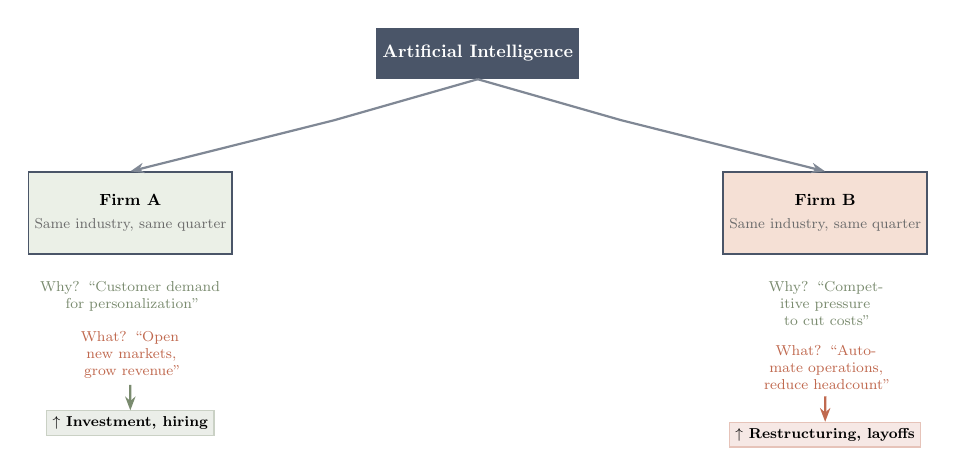
\begin{tikzpicture}[scale=0.65, every node/.style={transform shape, font=\small},
  firm/.style={rectangle, minimum width=3.2cm, minimum height=1.6cm, draw=slate, line width=0.6pt, align=center},
  tech/.style={rectangle, minimum width=3cm, minimum height=1cm, fill=slate, text=white, font=\bfseries\normalsize, align=center},
  arrow/.style={-{Stealth[length=5pt]}, line width=0.8pt, color=slate!70},
  cause/.style={font=\footnotesize, text=sage, align=center},
  effect/.style={font=\footnotesize, text=terracotta, align=center},
]

% Technology node at top
\node[tech] (ai) {Artificial Intelligence};

% Firm A — left
\node[firm, fill=sagefill, below left=1.8cm and 2.8cm of ai] (firmA) {
  \textbf{Firm A}\\[2pt]
  \footnotesize\textcolor{textlight}{Same industry, same quarter}
};

% Firm B — right
\node[firm, fill=terracottafill, below right=1.8cm and 2.8cm of ai] (firmB) {
  \textbf{Firm B}\\[2pt]
  \footnotesize\textcolor{textlight}{Same industry, same quarter}
};

% Arrows from tech to firms
\draw[arrow] (ai.south) -- ++(-2.8cm,-0.8cm) -- (firmA.north);
\draw[arrow] (ai.south) -- ++(2.8cm,-0.8cm) -- (firmB.north);

% Cause labels — stacked below firms with clear spacing
\node[cause, below=0.4cm of firmA, text width=3.5cm] (causeA) {
  \accent{Why?} ``Customer demand\\for personalization''
};
\node[effect, below=0.15cm of causeA, text width=3.5cm] (effectA) {
  \pop{What?} ``Open new markets,\\grow revenue''
};

\node[cause, below=0.4cm of firmB, text width=3.5cm] (causeB) {
  \accent{Why?} ``Competitive pressure\\to cut costs''
};
\node[effect, below=0.15cm of causeB, text width=3.5cm] (effectB) {
  \pop{What?} ``Automate operations,\\reduce headcount''
};

% Action boxes
\node[rectangle, fill=sage!15, draw=sage!40, minimum width=2.5cm, font=\footnotesize\bfseries, below=0.5cm of effectA] (actA) {$\uparrow$ Investment, hiring};
\node[rectangle, fill=terracotta!15, draw=terracotta!40, minimum width=2.5cm, font=\footnotesize\bfseries, below=0.5cm of effectB] (actB) {$\uparrow$ Restructuring, layoffs};

\draw[arrow, sage] (effectA.south) -- (actA.north);
\draw[arrow, terracotta] (effectB.south) -- (actB.north);

\end{tikzpicture}

\source{Illustrative. The paper measures this heterogeneity at scale across 29 technologies.}
\end{frame}


%---------- THE GAP ----------
\begin{frame}{What existing measures miss}
\centering
\vspace{10pt}
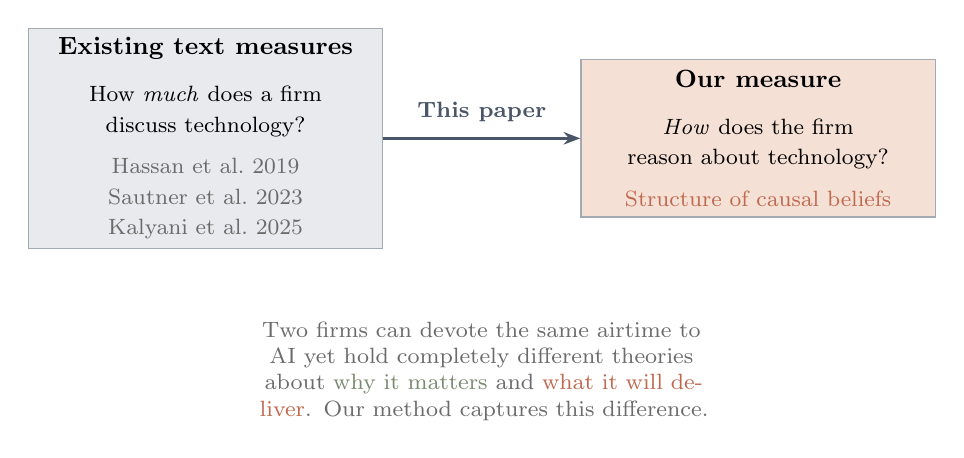
\begin{tikzpicture}[
  every node/.style={font=\small},
  box/.style={rectangle, minimum width=4.5cm, minimum height=2cm, align=center, draw=slate!50, line width=0.5pt},
]

% Existing measures
\node[box, fill=slatefill] (old) {
  \textbf{Existing text measures}\\[6pt]
  \footnotesize How \emph{much} does a firm\\
  \footnotesize discuss technology?\\[4pt]
  \footnotesize \gray{Hassan et al.\ 2019}\\
  \footnotesize \gray{Sautner et al.\ 2023}\\
  \footnotesize \gray{Kalyani et al.\ 2025}
};

% Our measure
\node[box, fill=terracottafill, right=2.5cm of old] (new) {
  \textbf{Our measure}\\[6pt]
  \footnotesize \emph{How} does the firm\\
  \footnotesize reason about technology?\\[4pt]
  \footnotesize \pop{Structure of causal beliefs}
};

% Arrow
\draw[-{Stealth[length=6pt]}, line width=1.2pt, slate] (old.east) -- node[above, font=\footnotesize\bfseries, yshift=2pt] {This paper} (new.west);

% Annotation below
\node[below=1cm of $(old.south)!0.5!(new.south)$, font=\footnotesize, text=textlight, align=center, text width=10cm] {
  Two firms can devote the same airtime to AI yet hold completely different theories\\
  about \accent{why it matters} and \pop{what it will deliver}. Our method captures this difference.
};

\end{tikzpicture}
\end{frame}


%---------- ONE-SENTENCE PITCH ----------
\begin{frame}{In one sentence}
\centering
\vfill
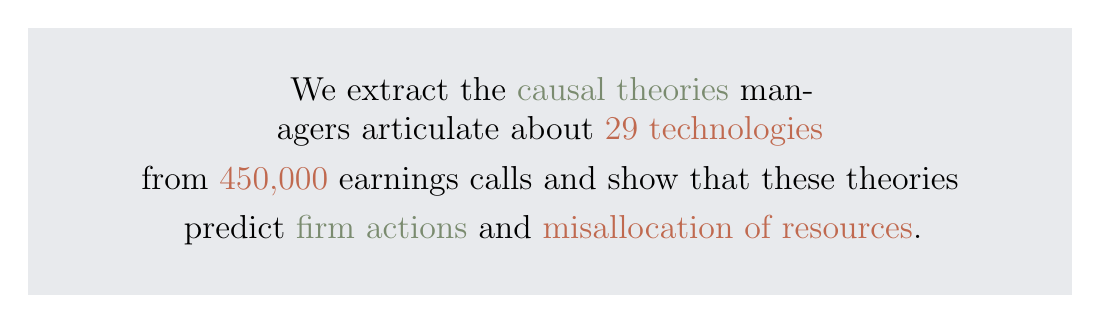
\begin{tikzpicture}
\node[rectangle, fill=slatefill, inner sep=18pt, text width=12cm, align=center, font=\large] {
  We extract the \accent{causal theories} managers articulate about \pop{29 technologies}\\[4pt]
  from \pop{450,000} earnings calls and show that these theories\\[4pt]
  predict \accent{firm actions} and \pop{misallocation of resources}.
};
\end{tikzpicture}
\vfill
\end{frame}


%=============================================================
%  PART 2 — THE DATA AND MEASUREMENT
%=============================================================
\begin{transitionframe}
\centering
\vfill
{\color{white}\LARGE\bfseries Data and Measurement}\\[10pt]
{\color{white!65}\normalsize From earnings calls to a panel of causal beliefs}
\vfill
\end{transitionframe}


%---------- SCOPE ----------
\begin{frame}{Scale of the data}
\centering
\vspace{4pt}
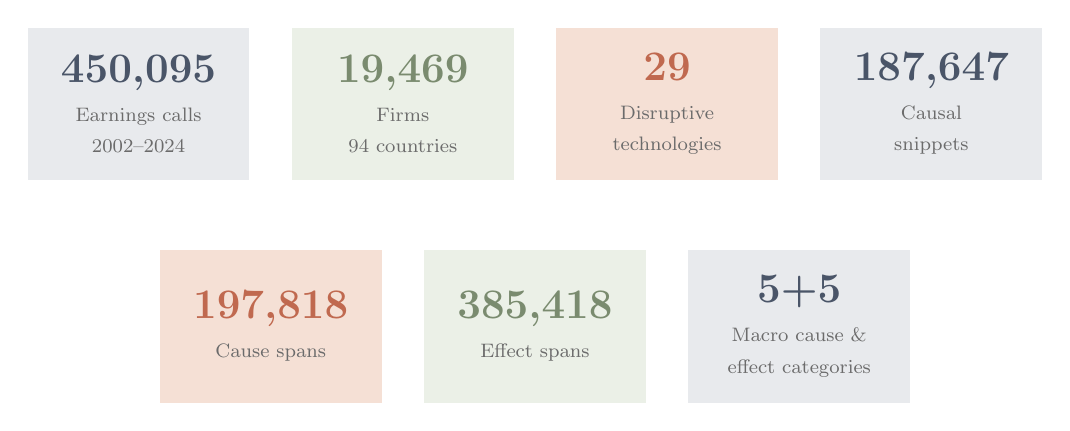
\begin{tikzpicture}[scale=0.88, every node/.style={transform shape},
]
\node[statslate] (n1) at (0,0) {\textcolor{slate}{\LARGE\bfseries 450,095}\\[4pt] {\footnotesize\textcolor{textlight}{Earnings calls}}\\[1pt]{\footnotesize\textcolor{textlight}{2002--2024}}};
\node[statsage, right=0.6cm of n1] (n2) {\textcolor{sage}{\LARGE\bfseries 19,469}\\[4pt] {\footnotesize\textcolor{textlight}{Firms}}\\[1pt]{\footnotesize\textcolor{textlight}{94 countries}}};
\node[statterracotta, right=0.6cm of n2] (n3) {\textcolor{terracotta}{\LARGE\bfseries 29}\\[4pt] {\footnotesize\textcolor{textlight}{Disruptive}}\\[1pt]{\footnotesize\textcolor{textlight}{technologies}}};
\node[statslate, right=0.6cm of n3] (n4) {\textcolor{slate}{\LARGE\bfseries 187,647}\\[4pt] {\footnotesize\textcolor{textlight}{Causal}}\\[1pt]{\footnotesize\textcolor{textlight}{snippets}}};

% bottom row
\node[statterracotta, below=1cm of $(n1.south)!0.5!(n2.south)$] (n5) {\textcolor{terracotta}{\LARGE\bfseries 197,818}\\[4pt] {\footnotesize\textcolor{textlight}{Cause spans}}};
\node[statsage, right=0.6cm of n5] (n6) {\textcolor{sage}{\LARGE\bfseries 385,418}\\[4pt] {\footnotesize\textcolor{textlight}{Effect spans}}};
\node[statslate, right=0.6cm of n6] (n7) {\textcolor{slate}{\LARGE\bfseries 5+5}\\[4pt] {\footnotesize\textcolor{textlight}{Macro cause \&}}\\[1pt]{\footnotesize\textcolor{textlight}{effect categories}}};
\end{tikzpicture}

\source{Technologies from Kalyani et al.\ (2025, QJE). Transcripts from Refinitiv Eikon.}
\end{frame}


%---------- PIPELINE FIGURE ----------
\begin{frame}{The measurement pipeline}
\centering
\vspace{-2pt}
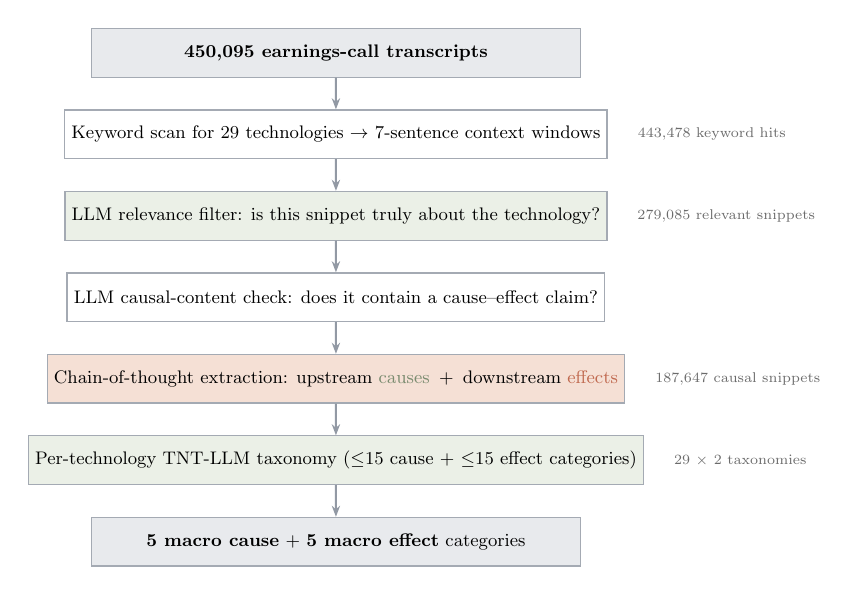
\begin{tikzpicture}[
  scale=0.73, every node/.style={transform shape},
  arr/.style={-{Stealth[length=4pt]}, line width=0.7pt, slate!60},
  side/.style={font=\scriptsize, text=textlight, align=left},
  node distance=0.55cm,
]

\node[stepslatefill] (s1) {\textbf{450,095 earnings-call transcripts}};
\node[stepwhite, below=of s1] (s2) {Keyword scan for 29 technologies $\rightarrow$ 7-sentence context windows};
\node[stepsagefill, below=of s2] (s3) {LLM relevance filter: is this snippet truly about the technology?};
\node[stepwhite, below=of s3] (s4) {LLM causal-content check: does it contain a cause--effect claim?};
\node[steptcfill, below=of s4] (s5) {Chain-of-thought extraction: upstream \accent{causes} $\,+\,$ downstream \pop{effects}};
\node[stepsagefill, below=of s5] (s6) {Per-technology TNT-LLM taxonomy ($\leq$15 cause $+$ $\leq$15 effect categories)};
\node[stepslatefill, below=of s6] (s7) {\textbf{5 macro cause} $+$ \textbf{5 macro effect} categories};

\draw[arr] (s1) -- (s2);
\draw[arr] (s2) -- (s3);
\draw[arr] (s3) -- (s4);
\draw[arr] (s4) -- (s5);
\draw[arr] (s5) -- (s6);
\draw[arr] (s6) -- (s7);

% side annotations
\node[side, right=0.4cm of s2] {443,478 keyword hits};
\node[side, right=0.4cm of s3] {279,085 relevant snippets};
\node[side, right=0.4cm of s5] {187,647 causal snippets};
\node[side, right=0.4cm of s6] {29 $\times$ 2 taxonomies};

\end{tikzpicture}
\end{frame}


%---------- WHAT IS A CAUSAL THEORY ----------
\begin{frame}{What is a ``causal theory''?}
\centering
\vspace{8pt}
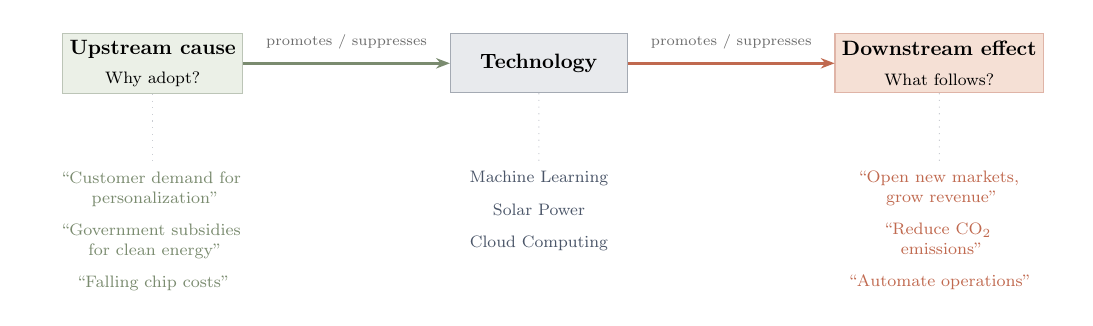
\begin{tikzpicture}[scale=0.75, every node/.style={transform shape, font=\small},
  box/.style={rectangle, minimum width=3cm, minimum height=1cm, align=center, font=\normalsize},
  arr/.style={-{Stealth[length=5pt]}, line width=1pt},
]

% Top: conceptual — wider spacing so labels fit
\node[box, fill=sagefill, draw=sage!50] (cause) {\textbf{Upstream cause}\\[2pt]\footnotesize Why adopt?};
\node[box, fill=slatefill, draw=slate!50, right=3.5cm of cause] (tech) {\textbf{Technology}};
\node[box, fill=terracottafill, draw=terracotta!50, right=3.5cm of tech] (effect) {\textbf{Downstream effect}\\[2pt]\footnotesize What follows?};

\draw[arr, sage] (cause) -- node[above, font=\scriptsize, text=textlight, yshift=3pt] {promotes / suppresses} (tech);
\draw[arr, terracotta] (tech) -- node[above, font=\scriptsize, text=textlight, yshift=3pt] {promotes / suppresses} (effect);

% Examples below
\node[below=1.2cm of cause, font=\footnotesize, text=sage, align=center, text width=4cm] (ex1) {
  ``Customer demand for\\personalization''\\[6pt]
  ``Government subsidies\\for clean energy''\\[6pt]
  ``Falling chip costs''
};

\node[below=1.2cm of tech, font=\footnotesize, text=slate, align=center] (ex2) {
  Machine Learning\\[6pt]
  Solar Power\\[6pt]
  Cloud Computing
};

\node[below=1.2cm of effect, font=\footnotesize, text=terracotta, align=center, text width=4cm] (ex3) {
  ``Open new markets,\\grow revenue''\\[6pt]
  ``Reduce CO\textsubscript{2}\\emissions''\\[6pt]
  ``Automate operations''
};

% Connecting lines
\draw[dotted, slate!30] (cause.south) -- (ex1.north);
\draw[dotted, slate!30] (tech.south) -- (ex2.north);
\draw[dotted, slate!30] (effect.south) -- (ex3.north);

\end{tikzpicture}
\source{Each extracted triple: (cause, promotes/suppresses, technology) or (technology, promotes/suppresses, effect).}
\end{frame}


%---------- MACRO CATEGORIES VISUAL ----------
\begin{frame}{The taxonomy: 5 causes $\times$ 5 effects}
\centering
\vspace{2pt}
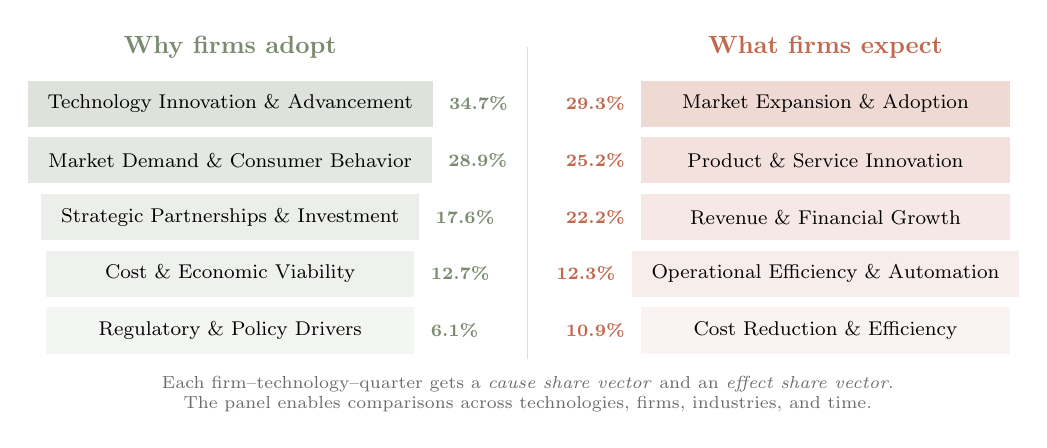
\begin{tikzpicture}[scale=0.9, every node/.style={transform shape, font=\footnotesize},
  catbox/.style={rectangle, minimum width=5.2cm, minimum height=0.65cm, align=left, inner xsep=8pt},
  pctlabel/.style={font=\scriptsize\bfseries},
]

% CAUSES — left column
\node[font=\normalsize\bfseries, text=sage] at (-4.2, 3.6) {Why firms adopt};
\node[catbox, fill=sage!25] (c1) at (-4.2, 2.8) {Technology Innovation \& Advancement};
\node[pctlabel, right=0.1cm of c1, text=sage] {34.7\%};
\node[catbox, fill=sage!20] (c2) at (-4.2, 2.0) {Market Demand \& Consumer Behavior};
\node[pctlabel, right=0.1cm of c2, text=sage] {28.9\%};
\node[catbox, fill=sage!15] (c3) at (-4.2, 1.2) {Strategic Partnerships \& Investment};
\node[pctlabel, right=0.1cm of c3, text=sage] {17.6\%};
\node[catbox, fill=sage!12] (c4) at (-4.2, 0.4) {Cost \& Economic Viability};
\node[pctlabel, right=0.1cm of c4, text=sage] {12.7\%};
\node[catbox, fill=sage!8] (c5) at (-4.2, -0.4) {Regulatory \& Policy Drivers};
\node[pctlabel, right=0.1cm of c5, text=sage] {6.1\%};

% EFFECTS — right column
\node[font=\normalsize\bfseries, text=terracotta] at (4.2, 3.6) {What firms expect};
\node[catbox, fill=terracotta!25] (e1) at (4.2, 2.8) {Market Expansion \& Adoption};
\node[pctlabel, left=0.1cm of e1, text=terracotta] {29.3\%};
\node[catbox, fill=terracotta!20] (e2) at (4.2, 2.0) {Product \& Service Innovation};
\node[pctlabel, left=0.1cm of e2, text=terracotta] {25.2\%};
\node[catbox, fill=terracotta!15] (e3) at (4.2, 1.2) {Revenue \& Financial Growth};
\node[pctlabel, left=0.1cm of e3, text=terracotta] {22.2\%};
\node[catbox, fill=terracotta!12] (e4) at (4.2, 0.4) {Operational Efficiency \& Automation};
\node[pctlabel, left=0.1cm of e4, text=terracotta] {12.3\%};
\node[catbox, fill=terracotta!8] (e5) at (4.2, -0.4) {Cost Reduction \& Efficiency};
\node[pctlabel, left=0.1cm of e5, text=terracotta] {10.9\%};

% Central divider
\draw[slate!20, line width=0.4pt] (0, 3.6) -- (0, -0.8);

% Bottom annotation
\node[font=\scriptsize, text=textlight, align=center] at (0, -1.3) {
  Each firm--technology--quarter gets a \emph{cause share vector} and an \emph{effect share vector}.\\
  The panel enables comparisons across technologies, firms, industries, and time.
};

\end{tikzpicture}
\end{frame}


%---------- CROSS-TECH VALIDATION ----------
\begin{frame}{Face validity: cause profiles vary as expected}
\centering
\vspace{4pt}
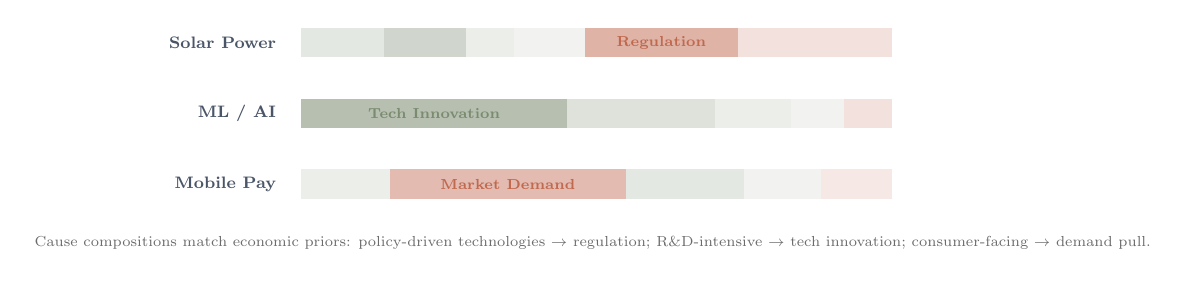
\begin{tikzpicture}[scale=0.75, every node/.style={transform shape, font=\small},
  techlab/.style={font=\footnotesize\bfseries, text=slate},
  bar/.style={rectangle, minimum height=0.4cm, inner sep=0pt, anchor=west},
  pct/.style={font=\tiny, text=textlight},
]

% Helper for stacked bars
% We'll draw simplified horizontal stacked bars for 3 technologies

% --- Solar Power ---
\node[techlab, anchor=east] at (-0.3, 2.4) {Solar Power};
% Regulation heavy
\fill[sage!20] (0, 2.15) rectangle (1.4, 2.65);     % Tech Innov 14%
\fill[sage!35] (1.4, 2.15) rectangle (2.8, 2.65);    % Market Demand 14%
\fill[sage!15] (2.8, 2.15) rectangle (3.6, 2.65);    % Strategic 8%
\fill[sage!10] (3.6, 2.15) rectangle (4.8, 2.65);    % Cost 12%
\fill[terracotta!50] (4.8, 2.15) rectangle (7.4, 2.65);  % Regulation 26%  ← LARGE
\fill[terracotta!20] (7.4, 2.15) rectangle (10, 2.65);   % Other
\node[font=\scriptsize\bfseries, text=terracotta] at (6.1, 2.4) {Regulation};

% --- ML / AI ---
\node[techlab, anchor=east] at (-0.3, 1.2) {ML / AI};
% Tech innovation heavy
\fill[sage!55] (0, 0.95) rectangle (4.5, 1.45);      % Tech Innov 45% ← LARGE
\fill[sage!25] (4.5, 0.95) rectangle (7.0, 1.45);    % Market Demand 25%
\fill[sage!15] (7.0, 0.95) rectangle (8.3, 1.45);    % Strategic 13%
\fill[sage!10] (8.3, 0.95) rectangle (9.2, 1.45);    % Cost 9%
\fill[terracotta!20] (9.2, 0.95) rectangle (10, 1.45);  % Regulation 8%
\node[font=\scriptsize\bfseries, text=sage] at (2.25, 1.2) {Tech Innovation};

% --- Mobile Payments ---
\node[techlab, anchor=east] at (-0.3, 0.0) {Mobile Pay};
% Demand heavy
\fill[sage!15] (0, -0.25) rectangle (1.5, 0.25);     % Tech Innov 15%
\fill[terracotta!45] (1.5, -0.25) rectangle (5.5, 0.25);  % Market Demand 40% ← LARGE
\fill[sage!20] (5.5, -0.25) rectangle (7.5, 0.25);   % Strategic 20%
\fill[sage!10] (7.5, -0.25) rectangle (8.8, 0.25);   % Cost 13%
\fill[terracotta!15] (8.8, -0.25) rectangle (10, 0.25);  % Regulation 12%
\node[font=\scriptsize\bfseries, text=terracotta] at (3.5, 0.0) {Market Demand};

% Legend at bottom
\node[font=\scriptsize, text=textlight, align=center] at (5, -1.0) {
  Cause compositions match economic priors: policy-driven technologies $\rightarrow$ regulation;
  R\&D-intensive $\rightarrow$ tech innovation; consumer-facing $\rightarrow$ demand pull.
};

\end{tikzpicture}
\source{Stylized representation of aggregate macro-cause shares by technology.}
\end{frame}


%=============================================================
%  PART 3 — THE FOUR FINDINGS
%=============================================================
\begin{transitionframepop}
\centering
\vfill
{\color{white}\LARGE\bfseries Four Main Findings}
\vfill
\end{transitionframepop}


%---------- FINDING 1: FIRM-LEVEL HETEROGENEITY ----------
\begin{frame}{Finding 1: Most variation is at the firm level}
\centering
\vspace{4pt}
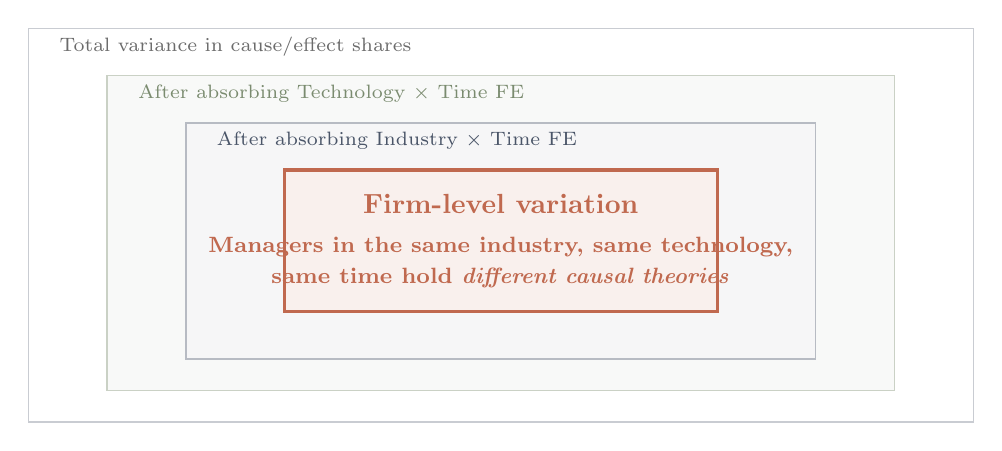
\begin{tikzpicture}[
  every node/.style={font=\small},
]

% Variance decomposition as nested boxes
% Outermost = total variance
\node[rectangle, draw=slate!30, line width=0.5pt, minimum width=12cm, minimum height=5cm, fill=white] (total) {};
\node[font=\scriptsize, text=textlight, anchor=north west] at (total.north west) {\quad Total variance in cause/effect shares};

% Technology × Time
\node[rectangle, draw=sage!40, line width=0.5pt, minimum width=10cm, minimum height=4cm, fill=sage!5, anchor=north] at ([yshift=-0.6cm]total.north) (techtime) {};
\node[font=\scriptsize, text=sage, anchor=north west] at (techtime.north west) {\quad After absorbing Technology $\times$ Time FE};

% Industry × Time
\node[rectangle, draw=slate!40, line width=0.5pt, minimum width=8cm, minimum height=3cm, fill=slate!5, anchor=north] at ([yshift=-0.6cm]techtime.north) (indtime) {};
\node[font=\scriptsize, text=slate, anchor=north west] at (indtime.north west) {\quad After absorbing Industry $\times$ Time FE};

% Firm FE — the big remaining piece
\node[rectangle, draw=terracotta, line width=1.2pt, minimum width=5.5cm, minimum height=1.8cm, fill=terracotta!10, anchor=center] at (indtime.center) (firm) {};
\node[font=\normalsize\bfseries, text=terracotta, align=center] at (firm.center) {
  Firm-level variation\\[2pt]
  \footnotesize Managers in the same industry, same technology,\\[-1pt]
  \footnotesize same time hold \emph{different causal theories}
};

\end{tikzpicture}

\source{Parallels Hassan et al.\ (2019): most political risk variation is firm-level. Here the object is belief \emph{structure}, not attention.}
\end{frame}


%---------- FINDING 2: PORTABLE BELIEFS ----------
\begin{frame}{Finding 2: Beliefs are persistent and portable}
\vspace{4pt}
\begin{columns}[T]
\begin{column}{0.42\textwidth}
\centering
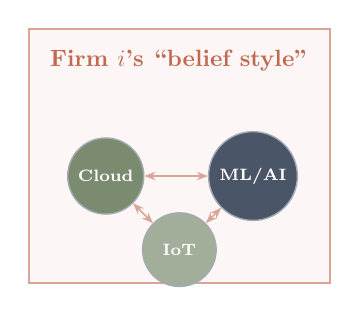
\begin{tikzpicture}[scale=0.85, every node/.style={transform shape, font=\small}]

% Firm box
\node[rectangle, draw=terracotta!60, line width=0.8pt, fill=terracotta!5, minimum width=4.5cm, minimum height=3.8cm, align=center] (firm) {};
\node[font=\normalsize\bfseries, text=terracotta, anchor=north] at ([yshift=-6pt]firm.north) {Firm $i$'s ``belief style''};

% Technologies inside firm
\node[circle, minimum size=1.1cm, draw=slate!50, line width=0.5pt, fill=sage, font=\scriptsize\bfseries, align=center, text=white] (t1) at ([xshift=-1.1cm, yshift=-0.3cm]firm.center) {Cloud};
\node[circle, minimum size=1.1cm, draw=slate!50, line width=0.5pt, fill=slate, font=\scriptsize\bfseries, align=center, text=white] (t2) at ([xshift=1.1cm, yshift=-0.3cm]firm.center) {ML/AI};
\node[circle, minimum size=1.1cm, draw=slate!50, line width=0.5pt, fill=sage!70, font=\scriptsize\bfseries, align=center, text=white] (t3) at ([xshift=0cm, yshift=-1.4cm]firm.center) {IoT};

% Arrows showing same frame
\draw[{Stealth[length=4pt]}-{Stealth[length=4pt]}, terracotta!60, line width=0.6pt] (t1) -- (t2);
\draw[{Stealth[length=4pt]}-{Stealth[length=4pt]}, terracotta!60, line width=0.6pt] (t1) -- (t3);
\draw[{Stealth[length=4pt]}-{Stealth[length=4pt]}, terracotta!60, line width=0.6pt] (t2) -- (t3);

\end{tikzpicture}
\end{column}
\begin{column}{0.55\textwidth}
\begin{wideitemize}
  \item A firm whose cloud narrative emphasizes \accent{market demand} as the adoption driver also frames ML/AI in \accent{demand-pull} terms.
  \item When a firm starts discussing a \emph{new} technology, its initial frame resembles the frame for technologies it already discusses.
  \item Consistent with \pop{diagnostic expectations}: agents overweight salient features of past experience.\\[2pt]
  \gray{Bordalo, Gennaioli \& Shleifer (2018)}
\end{wideitemize}
\end{column}
\end{columns}
\end{frame}


%---------- FINDING 3: BELIEFS PREDICT ACTIONS ----------
\begin{frame}{Finding 3: Beliefs predict firm actions}
\centering
\vspace{2pt}
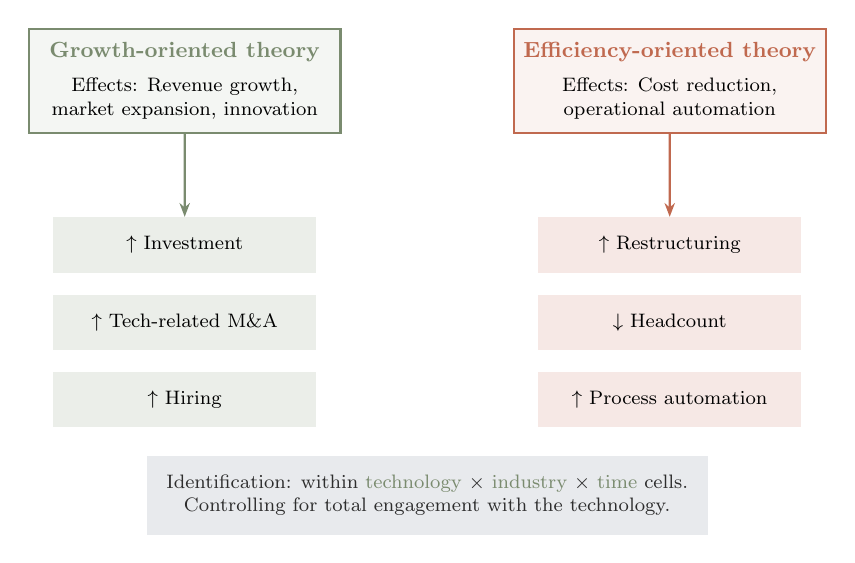
\begin{tikzpicture}[scale=0.88, every node/.style={transform shape, font=\small},
]

% Growth theory
\node[theorysage] (growth) at (-3.5, 1.5) {
  \textbf{\textcolor{sage}{Growth-oriented theory}}\\[3pt]
  \footnotesize Effects: Revenue growth,\\[-1pt]
  \footnotesize market expansion, innovation
};

% Efficiency theory
\node[theorytc] (effic) at (3.5, 1.5) {
  \textbf{\textcolor{terracotta}{Efficiency-oriented theory}}\\[3pt]
  \footnotesize Effects: Cost reduction,\\[-1pt]
  \footnotesize operational automation
};

% Actions
\node[actsage, below=1.2cm of growth] (act1) {$\uparrow$ Investment};
\node[actsage, below=0.3cm of act1] (act2) {$\uparrow$ Tech-related M\&A};
\node[actsage, below=0.3cm of act2] (act3) {$\uparrow$ Hiring};

\node[acttc, below=1.2cm of effic] (act4) {$\uparrow$ Restructuring};
\node[acttc, below=0.3cm of act4] (act5) {$\downarrow$ Headcount};
\node[acttc, below=0.3cm of act5] (act6) {$\uparrow$ Process automation};

% Arrows
\draw[-{Stealth[length=5pt]}, line width=0.8pt, sage] (growth.south) -- (act1.north);
\draw[-{Stealth[length=5pt]}, line width=0.8pt, terracotta] (effic.south) -- (act4.north);

% Identification note
\node[rectangle, fill=slatefill, inner sep=8pt, font=\footnotesize, text=textmain, align=center, below=0.4cm of $(act3.south)!0.5!(act6.south)$] {
  Identification: within \accent{technology} $\times$ \accent{industry} $\times$ \accent{time} cells.\\
  Controlling for total engagement with the technology.
};

\end{tikzpicture}
\end{frame}


%---------- FINDING 4: MISALLOCATION ----------
\begin{frame}{Finding 4: Wrong theories $\rightarrow$ worse outcomes}
\centering
\vspace{2pt}
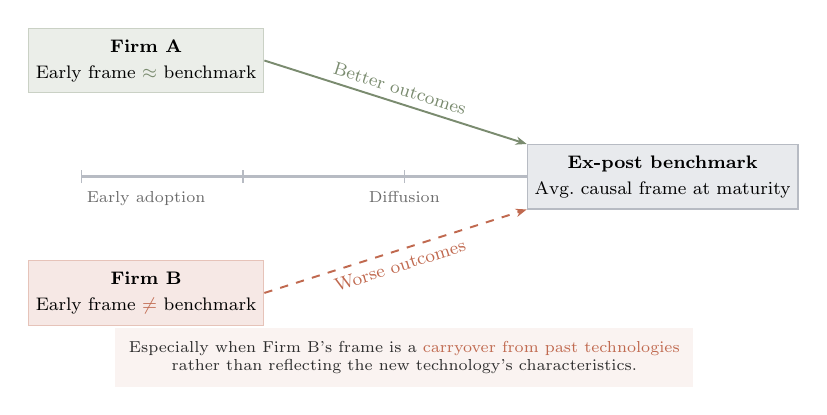
\begin{tikzpicture}[scale=0.82, every node/.style={transform shape, font=\small},
  node distance=0.8cm,
]

% Timeline
\draw[slate!40, line width=1pt] (0, 0) -- (10, 0);

% Time markers
\node[below=3pt, font=\scriptsize, text=textlight] at (1, 0) {Early adoption};
\node[below=3pt, font=\scriptsize, text=textlight] at (5, 0) {Diffusion};
\node[below=3pt, font=\scriptsize, text=textlight] at (9, 0) {Maturity};

% Ticks
\foreach \x in {0, 2.5, 5, 7.5, 10} {
  \draw[slate!40, line width=0.5pt] (\x, -0.1) -- (\x, 0.1);
}

% Firm A — aligned with eventual trajectory
\node[rectangle, fill=sage!15, draw=sage!40, minimum width=2.4cm, minimum height=1cm, align=center, font=\footnotesize] at (1, 1.8) (fA) {
  \textbf{Firm A}\\[2pt]
  Early frame \accent{$\approx$} benchmark
};

% Firm B — misaligned
\node[rectangle, fill=terracotta!15, draw=terracotta!40, minimum width=2.4cm, minimum height=1cm, align=center, font=\footnotesize] at (1, -1.8) (fB) {
  \textbf{Firm B}\\[2pt]
  Early frame \pop{$\neq$} benchmark
};

% Benchmark
\node[rectangle, fill=slatefill, draw=slate!40, minimum width=2.4cm, minimum height=1cm, align=center, font=\footnotesize] at (9, 0.0) (bench) {
  \textbf{Ex-post benchmark}\\[2pt]
  Avg.\ causal frame at maturity
};

% Arrows from firms to benchmark
\draw[-{Stealth[length=4pt]}, sage, line width=0.7pt] (fA.east) -- (bench.north west) node[above, midway, font=\footnotesize, text=sage, sloped] {Better outcomes};
\draw[-{Stealth[length=4pt]}, terracotta, line width=0.7pt, dashed] (fB.east) -- (bench.south west) node[below, midway, font=\footnotesize, text=terracotta, sloped] {Worse outcomes};

% Annotation below
\node[rectangle, fill=terracotta!8, inner sep=6pt, font=\scriptsize, text=textmain, align=center] at (5, -2.8) {
  Especially when Firm B's frame is a \pop{carryover from past technologies}\\
  rather than reflecting the new technology's characteristics.
};

\end{tikzpicture}
\end{frame}


%=============================================================
%  PART 4 — EMPIRICAL AGENDA
%=============================================================
\begin{transitionframe}
\centering
\vfill
{\color{white}\LARGE\bfseries The Empirical Agenda}\\[10pt]
{\color{white!65}\normalsize What we need to show and why}
\vfill
\end{transitionframe}


%---------- ROADMAP ----------
\begin{frame}{Six empirical tasks}
\centering
\vspace{4pt}
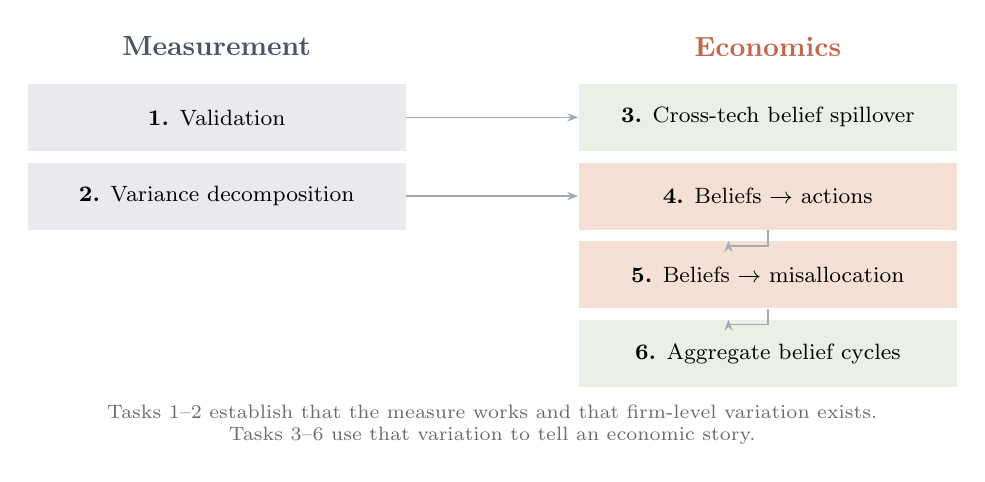
\begin{tikzpicture}[
  every node/.style={font=\small},
  arr/.style={-{Stealth[length=4pt]}, line width=0.6pt, slate!50},
]

% Left column — Measurement
\node[font=\normalsize\bfseries, text=slate] at (-3.5, 3.5) {Measurement};
\node[taskslatefill] (t1) at (-3.5, 2.6) {\textbf{1.} Validation};
\node[taskslatefill] (t2) at (-3.5, 1.6) {\textbf{2.} Variance decomposition};

% Right column — Economics
\node[font=\normalsize\bfseries, text=terracotta] at (3.5, 3.5) {Economics};
\node[tasksagefill] (t3) at (3.5, 2.6) {\textbf{3.} Cross-tech belief spillover};
\node[tasktcfill] (t4) at (3.5, 1.6) {\textbf{4.} Beliefs $\rightarrow$ actions};
\node[tasktcfill] (t5) at (3.5, 0.6) {\textbf{5.} Beliefs $\rightarrow$ misallocation};
\node[tasksagefill] (t6) at (3.5, -0.4) {\textbf{6.} Aggregate belief cycles};

% Dependency arrows
\draw[arr] (t1.east) -- ++(0.5,0) |- (t3.west);
\draw[arr] (t2.east) -- ++(0.3,0) |- (t4.west);
\draw[arr] (t4.south) -- ++(0, -0.2) -| ([xshift=-0.5cm]t5.north);
\draw[arr] (t5.south) -- ++(0, -0.2) -| ([xshift=-0.5cm]t6.north);

% Foundation label
\node[font=\scriptsize, text=textlight, align=center] at (0, -1.3) {
  Tasks 1--2 establish that the measure works and that firm-level variation exists.\\
  Tasks 3--6 use that variation to tell an economic story.
};

\end{tikzpicture}
\end{frame}


%---------- TASK 1: VALIDATION ----------
\begin{frame}{Task 1: Validation strategy}
\centering
\vspace{4pt}
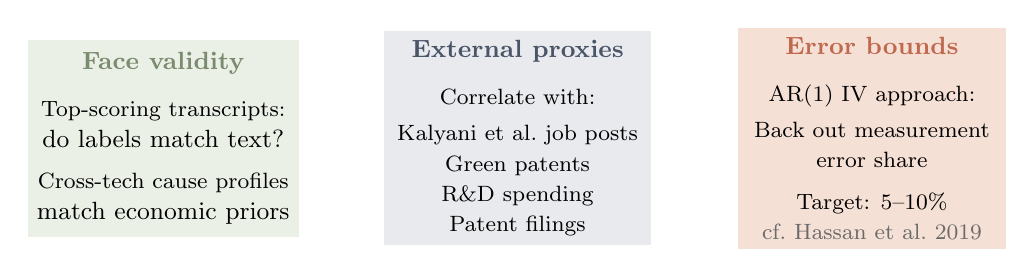
\begin{tikzpicture}[
  every node/.style={font=\small},
]

\node[vboxsage] (v1) at (0, 0) {
  \textbf{\textcolor{sage}{Face validity}}\\[6pt]
  \footnotesize Top-scoring transcripts:\\
  do labels match text?\\[4pt]
  \footnotesize Cross-tech cause profiles\\
  match economic priors
};

\node[vboxslate] (v2) at (4.5, 0) {
  \textbf{\textcolor{slate}{External proxies}}\\[6pt]
  \footnotesize Correlate with:\\[2pt]
  \footnotesize Kalyani et al.\ job posts\\
  \footnotesize Green patents\\
  \footnotesize R\&D spending\\
  \footnotesize Patent filings
};

\node[vboxtc] (v3) at (9, 0) {
  \textbf{\textcolor{terracotta}{Error bounds}}\\[6pt]
  \footnotesize AR(1) IV approach:\\[2pt]
  \footnotesize Back out measurement\\
  \footnotesize error share\\[4pt]
  \footnotesize Target: 5--10\%\\
  \footnotesize \gray{cf.\ Hassan et al.\ 2019}
};

\end{tikzpicture}
\source{Follows validation logic of Hassan et al.\ (2019, \S IV) and Sautner et al.\ (2023, \S III).}
\end{frame}


%---------- TASK 2: VARIANCE DECOMPOSITION ----------
\begin{frame}{Task 2: Variance decomposition}
\centering
\vspace{2pt}
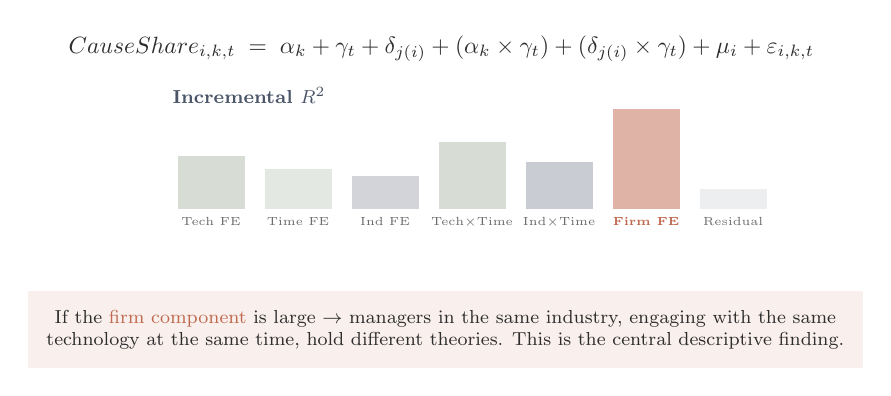
\begin{tikzpicture}[scale=0.85, every node/.style={transform shape, font=\small},
  fe/.style={rectangle, minimum width=2.2cm, minimum height=0.6cm, align=center, font=\footnotesize},
]

% The equation
\node[font=\normalsize, text=textmain, align=center] at (0, 3.4) {
  $\text{CauseShare}_{i,k,t} \;=\; \alpha_k + \gamma_t + \delta_{j(i)} + (\alpha_k \times \gamma_t) + (\delta_{j(i)} \times \gamma_t) + \mu_i + \varepsilon_{i,k,t}$
};

% Incremental R² label — left-aligned above bars, clear of equation
\node[font=\footnotesize\bfseries, text=slate, anchor=west] at (-4.2, 2.7) {Incremental $R^2$};

% Bar chart
\fill[sage!30] (-4, 1.0) rectangle (-3, 1.8);  % Tech FE
\node[font=\tiny, text=textlight, below] at (-3.5, 1.0) {Tech FE};

\fill[sage!20] (-2.7, 1.0) rectangle (-1.7, 1.6);  % Time FE
\node[font=\tiny, text=textlight, below] at (-2.2, 1.0) {Time FE};

\fill[slate!25] (-1.4, 1.0) rectangle (-0.4, 1.5);  % Ind FE
\node[font=\tiny, text=textlight, below] at (-0.9, 1.0) {Ind FE};

\fill[sage!30] (-0.1, 1.0) rectangle (0.9, 2.0);    % Tech$\times$Time
\node[font=\tiny, text=textlight, below] at (0.4, 1.0) {Tech$\times$Time};

\fill[slate!30] (1.2, 1.0) rectangle (2.2, 1.7);   % Ind$\times$Time
\node[font=\tiny, text=textlight, below] at (1.7, 1.0) {Ind$\times$Time};

\fill[terracotta!50] (2.5, 1.0) rectangle (3.5, 2.5);  % Firm FE — tallest
\node[font=\tiny\bfseries, text=terracotta, below] at (3.0, 1.0) {Firm FE};

\fill[slate!10] (3.8, 1.0) rectangle (4.8, 1.3);   % Residual
\node[font=\tiny, text=textlight, below] at (4.3, 1.0) {Residual};

% Key insight
\node[rectangle, fill=terracotta!10, inner sep=8pt, font=\footnotesize, text=textmain, align=center] at (0, -0.8) {
  If the \pop{firm component} is large $\rightarrow$ managers in the same industry, engaging with the same\\
  technology at the same time, hold different theories. This is the central descriptive finding.
};

\end{tikzpicture}
\source{Format follows Hassan et al.\ (2019, Table VIII). Run at 2-, 3-, and 4-digit SIC levels.}
\end{frame}


%---------- TASK 3: SPILLOVER ----------
\begin{frame}{Task 3: Cross-technology belief spillover}
\centering
\vspace{6pt}
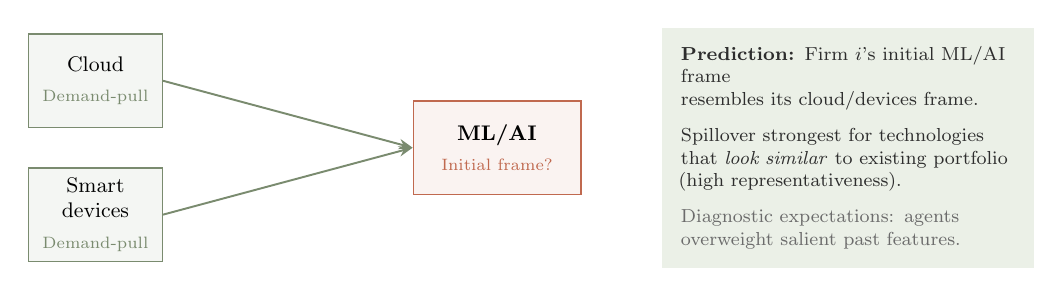
\begin{tikzpicture}[scale=0.85, every node/.style={transform shape, font=\small},
]

% Firm's existing portfolio
\node[framesage] (oldA) at (-4, 1) {Cloud\\[2pt]\scriptsize\accent{Demand-pull}};
\node[framesage] (oldB) at (-4, -1) {Smart\\devices\\[2pt]\scriptsize\accent{Demand-pull}};

% Arrow to new tech
\node[frametc, minimum width=2.5cm] (new) at (2, 0) {\textbf{ML/AI}\\[2pt]\scriptsize\pop{Initial frame?}};

\draw[-{Stealth[length=5pt]}, sage, line width=0.7pt] (oldA.east) -- (new.west);
\draw[-{Stealth[length=5pt]}, sage, line width=0.7pt] (oldB.east) -- (new.west);

% Prediction
\node[rectangle, fill=sagefill, inner sep=8pt, font=\footnotesize, text=textmain, align=left, text width=5cm, right=1.2cm of new] {
  \textbf{Prediction:} Firm $i$'s initial ML/AI frame\\
  resembles its cloud/devices frame.\\[6pt]
  Spillover strongest for technologies\\
  that \emph{look similar} to existing portfolio\\
  (high representativeness).\\[6pt]
  \gray{Diagnostic expectations: agents}\\
  \gray{overweight salient past features.}
};

\end{tikzpicture}
\source{Test: regress cause-share vector for tech $B$ on cause-share vector for tech $A$, absorbing tech and time FE.}
\end{frame}


%---------- TASK 4: BELIEFS → ACTIONS ----------
\begin{frame}{Task 4: Beliefs and actions}
\centering
\vspace{2pt}
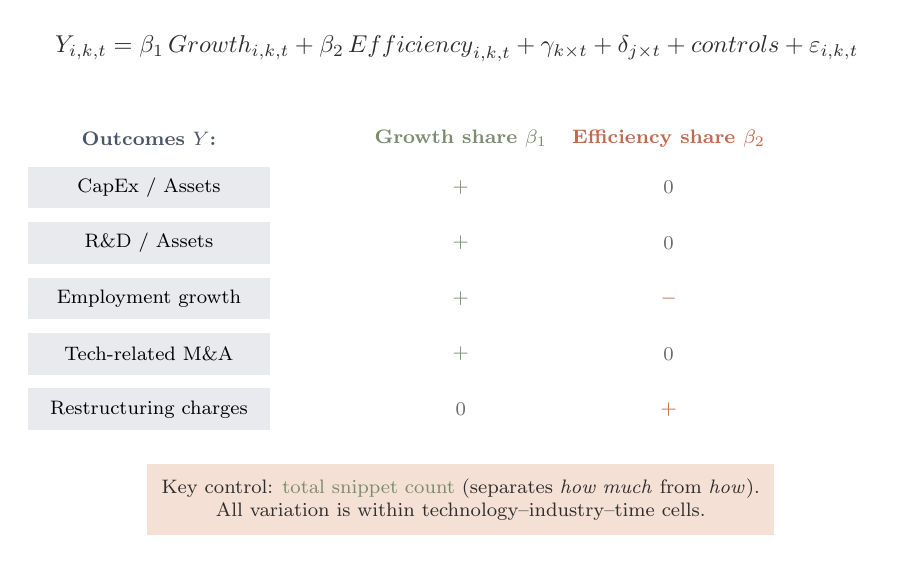
\begin{tikzpicture}[scale=0.88, every node/.style={transform shape, font=\small},
  lhs/.style={rectangle, fill=slatefill, minimum width=3.5cm, minimum height=0.6cm, font=\footnotesize, align=center},
]

% Equation
\node[font=\normalsize, text=textmain, align=center] at (0, 3.5) {
  $Y_{i,k,t} = \beta_1\,\text{Growth}_{i,k,t} + \beta_2\,\text{Efficiency}_{i,k,t} + \gamma_{k \times t} + \delta_{j \times t} + \text{controls} + \varepsilon_{i,k,t}$
};

% LHS outcomes
\node[font=\footnotesize\bfseries, text=slate] at (-4.5, 2.2) {Outcomes $Y$:};
\node[lhs] (y1) at (-4.5, 1.5) {CapEx / Assets};
\node[lhs] (y2) at (-4.5, 0.7) {R\&D / Assets};
\node[lhs] (y3) at (-4.5, -0.1) {Employment growth};
\node[lhs] (y4) at (-4.5, -0.9) {Tech-related M\&A};
\node[lhs] (y5) at (-4.5, -1.7) {Restructuring charges};

% Expected signs
\node[font=\footnotesize, text=sage, align=center] at (0, 2.2) {\textbf{Growth share $\beta_1$}};
\node[font=\footnotesize, text=sage] at (0, 1.5) {$+$};
\node[font=\footnotesize, text=sage] at (0, 0.7) {$+$};
\node[font=\footnotesize, text=sage] at (0, -0.1) {$+$};
\node[font=\footnotesize, text=sage] at (0, -0.9) {$+$};
\node[font=\footnotesize, text=textlight] at (0, -1.7) {$0$};

\node[font=\footnotesize, text=terracotta, align=center] at (3, 2.2) {\textbf{Efficiency share $\beta_2$}};
\node[font=\footnotesize, text=textlight] at (3, 1.5) {$0$};
\node[font=\footnotesize, text=textlight] at (3, 0.7) {$0$};
\node[font=\footnotesize, text=terracotta] at (3, -0.1) {$-$};
\node[font=\footnotesize, text=textlight] at (3, -0.9) {$0$};
\node[font=\footnotesize, text=terracotta] at (3, -1.7) {$+$};

% Key controls
\node[rectangle, fill=terracottafill, inner sep=6pt, font=\footnotesize, text=textmain, align=center] at (0, -3) {
  Key control: \accent{total snippet count} (separates \emph{how much} from \emph{how}).\\
  All variation is within technology--industry--time cells.
};

\end{tikzpicture}
\end{frame}


%---------- TASK 4B: DISAGREEMENT ----------
\begin{frame}{Manager--analyst disagreement}
\centering
\vspace{8pt}
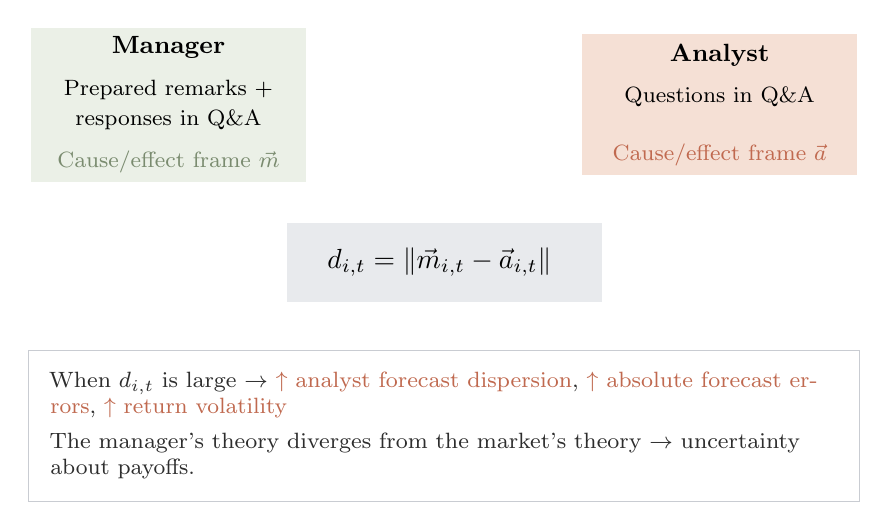
\begin{tikzpicture}[
  every node/.style={font=\small},
]

% Manager
\node[personsage] (mgr) at (-3.5, 1.5) {
  \textbf{Manager}\\[4pt]
  \footnotesize Prepared remarks $+$\\
  \footnotesize responses in Q\&A\\[4pt]
  \footnotesize \accent{Cause/effect frame $\vec{m}$}
};

% Analyst
\node[persontc] (ana) at (3.5, 1.5) {
  \textbf{Analyst}\\[4pt]
  \footnotesize Questions in Q\&A\\[10pt]
  \footnotesize \pop{Cause/effect frame $\vec{a}$}
};

% Disagreement
\node[rectangle, fill=slatefill, minimum width=4cm, minimum height=1cm, align=center, font=\normalsize] at (0, -0.5) (dis) {
  $d_{i,t} = \|\vec{m}_{i,t} - \vec{a}_{i,t}\|$
};

% Predictions
\node[rectangle, fill=white, draw=slate!30, inner sep=8pt, font=\footnotesize, text=textmain, align=left, text width=10cm, below=0.6cm of dis] {
  When $d_{i,t}$ is large $\rightarrow$ \pop{$\uparrow$ analyst forecast dispersion}, \pop{$\uparrow$ absolute forecast errors}, \pop{$\uparrow$ return volatility}\\[3pt]
  The manager's theory diverges from the market's theory $\rightarrow$ uncertainty about payoffs.
};

\end{tikzpicture}
\end{frame}


%---------- TASK 5: MISALLOCATION ----------
\begin{frame}{Task 5: Misallocation --- two identification strategies}
\centering
\vspace{2pt}
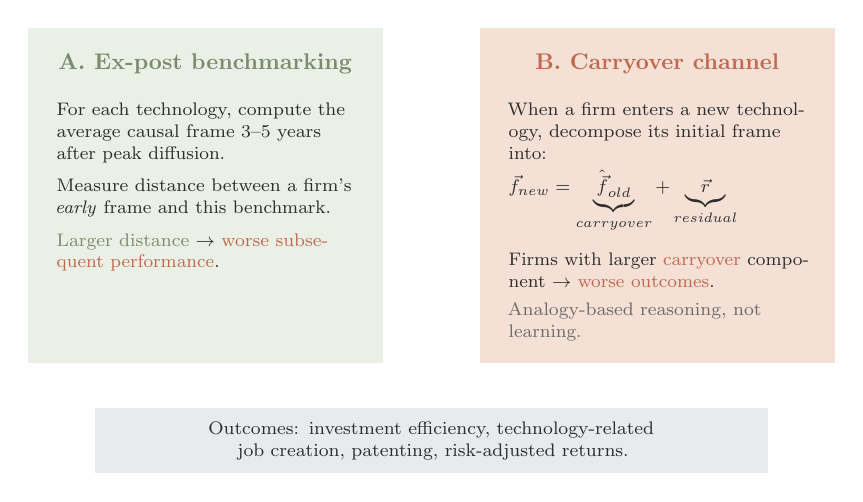
\begin{tikzpicture}[
  scale=0.82, every node/.style={transform shape, font=\small},
]

% Strategy A
\node[stratsage] (a) at (-3.5, 0) {};
\node[font=\normalsize\bfseries, text=sage, anchor=north] at ([yshift=-8pt]a.north) {A. Ex-post benchmarking};
\node[font=\footnotesize, text=textmain, align=left, text width=4.6cm, anchor=north] at ([yshift=-30pt]a.north) {
  For each technology, compute the
  average causal frame 3--5 years
  after peak diffusion.\\[5pt]
  Measure distance between a firm's
  \emph{early} frame and this benchmark.\\[5pt]
  \accent{Larger distance} $\rightarrow$ \pop{worse
  subsequent performance}.
};

% Strategy B
\node[strattc] (b) at (3.5, 0) {};
\node[font=\normalsize\bfseries, text=terracotta, anchor=north] at ([yshift=-8pt]b.north) {B. Carryover channel};
\node[font=\footnotesize, text=textmain, align=left, text width=4.6cm, anchor=north] at ([yshift=-30pt]b.north) {
  When a firm enters a new technology,
  decompose its initial frame into:\\[4pt]
  $\vec{f}_{new} = \underbrace{\hat{\vec{f}}_{old}}_{\text{carryover}} + \underbrace{\vec{r}}_{\text{residual}}$\\[8pt]
  Firms with larger \pop{carryover}
  component $\rightarrow$ \pop{worse outcomes}.\\[3pt]
  \gray{\footnotesize Analogy-based reasoning, not learning.}
};

% Outcomes — well below the boxes
\node[rectangle, fill=slatefill, inner sep=6pt, font=\footnotesize, text=textmain, align=center, text width=10cm] at (0, -3.8) {
  Outcomes: investment efficiency, technology-related job creation, patenting, risk-adjusted returns.
};

\end{tikzpicture}
\end{frame}


%---------- TASK 6: AGGREGATE CYCLES ----------
\begin{frame}{Task 6: Aggregate belief cycles}
\centering
\vspace{4pt}
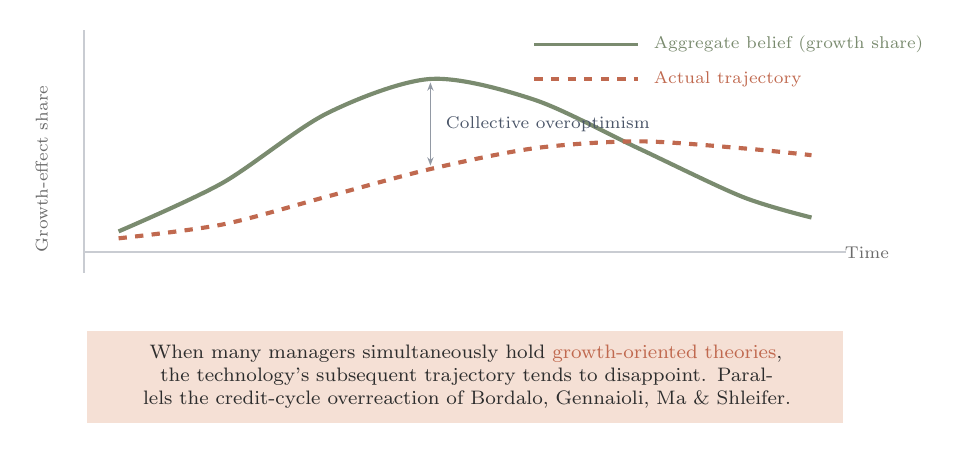
\begin{tikzpicture}[
  scale=0.88, every node/.style={transform shape, font=\small},
]

% Stylized belief cycle — axes
\draw[slate!30, line width=0.5pt] (0, 0) -- (11, 0);
\draw[slate!30, line width=0.5pt] (0, -0.3) -- (0, 3.2);

% Axis labels — placed clear of the annotation box
\node[font=\scriptsize, text=textlight, rotate=90, anchor=south] at (-0.4, 1.2) {Growth-effect share};
\node[font=\scriptsize, text=textlight] at (11.3, 0) {Time};

% The hump — aggregate belief
\draw[sage, line width=1.5pt, smooth] plot coordinates {
  (0.5, 0.3) (2, 1.0) (3.5, 2.0) (5, 2.5) (6.5, 2.2) (8, 1.5) (9.5, 0.8) (10.5, 0.5)
};

% Actual trajectory
\draw[terracotta, line width=1.5pt, dashed, smooth] plot coordinates {
  (0.5, 0.2) (2, 0.4) (3.5, 0.8) (5, 1.2) (6.5, 1.5) (8, 1.6) (9.5, 1.5) (10.5, 1.4)
};

% Legend — top right
\draw[sage, line width=1.2pt] (6.5, 3.0) -- (8, 3.0);
\node[font=\scriptsize, text=sage, anchor=west] at (8.1, 3.0) {Aggregate belief (growth share)};
\draw[terracotta, line width=1.2pt, dashed] (6.5, 2.5) -- (8, 2.5);
\node[font=\scriptsize, text=terracotta, anchor=west] at (8.1, 2.5) {Actual trajectory};

% Annotation: gap arrow
\draw[{Stealth[length=3pt]}-{Stealth[length=3pt]}, slate!60, line width=0.5pt] (5, 1.25) -- (5, 2.45);
\node[font=\scriptsize, text=slate, right] at (5.1, 1.85) {Collective overoptimism};

% Bottom text — placed well below axis
\node[rectangle, fill=terracottafill, inner sep=6pt, font=\footnotesize, text=textmain, align=center, text width=10.5cm] at (5.5, -1.8) {
  When many managers simultaneously hold \pop{growth-oriented theories}, the technology's
  subsequent trajectory tends to disappoint. Parallels the credit-cycle overreaction
  of Bordalo, Gennaioli, Ma \& Shleifer.
};

\end{tikzpicture}
\end{frame}


%=============================================================
%  CHALLENGES
%=============================================================
\begin{transitionframe}
\centering
\vfill
{\color{white}\LARGE\bfseries Challenges and Caveats}
\vfill
\end{transitionframe}


\begin{frame}{Identification threats and mitigations}
\centering
\vspace{6pt}
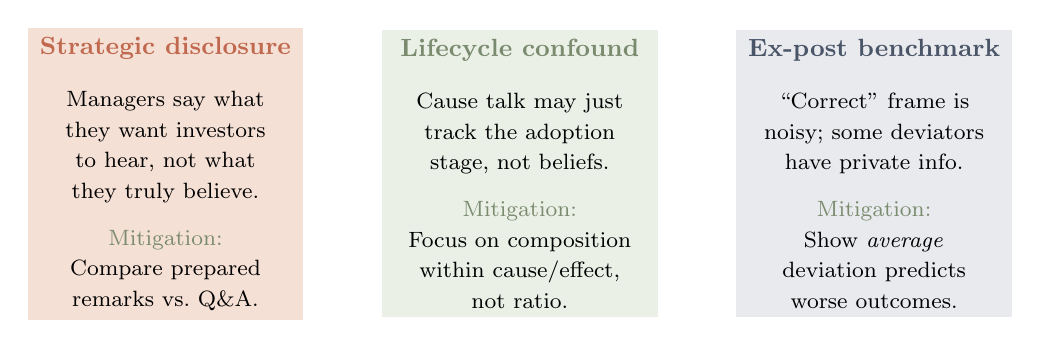
\begin{tikzpicture}[
  every node/.style={font=\small},
]

\node[risktc] (r1) at (-4.5, 0) {
  \textbf{\textcolor{terracotta}{Strategic disclosure}}\\[8pt]
  \footnotesize Managers say what\\
  \footnotesize they want investors\\
  \footnotesize to hear, not what\\
  \footnotesize they truly believe.\\[6pt]
  \footnotesize \accent{Mitigation:}\\
  \footnotesize Compare prepared\\
  \footnotesize remarks vs.\ Q\&A.
};

\node[risksage] (r2) at (0, 0) {
  \textbf{\textcolor{sage}{Lifecycle confound}}\\[8pt]
  \footnotesize Cause talk may just\\
  \footnotesize track the adoption\\
  \footnotesize stage, not beliefs.\\[6pt]
  \footnotesize \accent{Mitigation:}\\
  \footnotesize Focus on composition\\
  \footnotesize within cause/effect,\\
  \footnotesize not ratio.
};

\node[riskslate] (r3) at (4.5, 0) {
  \textbf{\textcolor{slate}{Ex-post benchmark}}\\[8pt]
  \footnotesize ``Correct'' frame is\\
  \footnotesize noisy; some deviators\\
  \footnotesize have private info.\\[6pt]
  \footnotesize \accent{Mitigation:}\\
  \footnotesize Show \emph{average}\\
  \footnotesize deviation predicts\\
  \footnotesize worse outcomes.
};

\end{tikzpicture}
\end{frame}


%=============================================================
%  CLOSING
%=============================================================
\begin{transitionframe}
\centering
\vfill
{\color{white}\LARGE\bfseries Summary}
\vfill
\end{transitionframe}


\begin{frame}{What this project delivers}
\centering
\vspace{6pt}
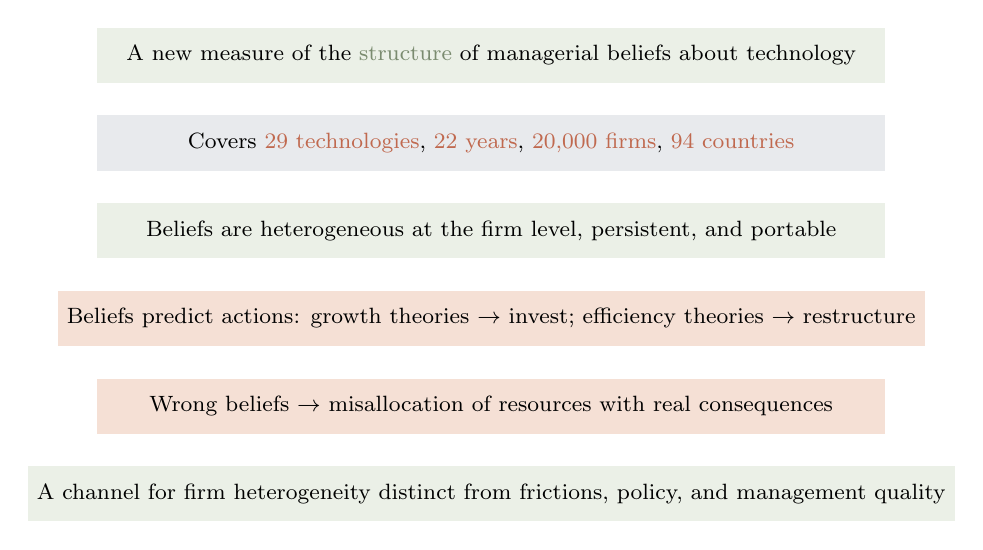
\begin{tikzpicture}[
  every node/.style={font=\small},
  node distance=0.4cm,
]

\node[itemsagefill] (d1) {A new measure of the \accent{structure} of managerial beliefs about technology};
\node[itemslatefill, below=of d1] (d2) {Covers \pop{29 technologies}, \pop{22 years}, \pop{20,000 firms}, \pop{94 countries}};
\node[itemsagefill, below=of d2] (d3) {Beliefs are heterogeneous at the firm level, persistent, and portable};
\node[itemtcfill, below=of d3] (d4) {Beliefs predict actions: growth theories $\rightarrow$ invest; efficiency theories $\rightarrow$ restructure};
\node[itemtcfill, below=of d4] (d5) {Wrong beliefs $\rightarrow$ misallocation of resources with real consequences};
\node[itemsagefill, below=of d5] (d6) {A channel for firm heterogeneity distinct from frictions, policy, and management quality};

\end{tikzpicture}
\end{frame}


\begin{transitionframe}
\centering
\vfill
{\color{white}\LARGE\bfseries Thank You}\\[12pt]
{\color{white!65}\normalsize lvanlent@fs.de}
\vfill
\end{transitionframe}


\end{document}
